% $Id$

\documentclass[a4paper,12pt]{article}

\setlength{\parindent}{0mm}
\setlength{\parskip}{7.5mm}

\usepackage[left=2cm,right=2cm,top=4cm,bottom=4cm]{geometry}
\usepackage{graphicx}

\begin{document}

\title{4ICT9 \\ Assignment 1}

\author{Conall O'Brien \\ 01734351 \\ conallob@maths.tcd.ie}

\maketitle

\section{Introduction}

Due to issues arising from being unable to form a group of 2 to 3 people to complete
this assignment, I ended up surveying the mobile network and writing
this report as an individual.


Hopefully, I shall clearly explain the route around the TCD campus and
the method used to conduct a survey. Then I shall analyse the data
collected in an effort to try to determine the physical locations of any
radio masts based upon mobile cell details.

\section{Surveying Campus}

Due to personal and professional reasons, I decided not to use my usual
Vodafone SIM card to perform the survey. Instead, I purchased a
disposable SIM card for the O2 network to conduct the survey.


Starting in the East End of the TCD Campus, I began taking readings
using the Nokia 3210 made available for the assignment. Included in this
document is a map of TCD campus with all 28 positions I took readings from.


The surveying was conducted in two outings, the first on Thursday
November 3rd between 11:00 and 12:30. Conditions deteriorated during the
survey. Initially, the weather was overcast and slightly windy, which
unsurprisingly resulted in rain and strong winds towards the end of the
session.


The second surveying outing was conducted on Friday November 11th,
between 16:00 and 17:30. During this outing, conditions were better than
the first, since there was no precipitation. However, due to the time of
the surveying, natural light was an issue, which affected my choices for
the last few surveying positions.

\subsection{Survey Details}

\subsection{Map of Survey Locations}

Please see figure 1.

\begin{figure}[h]

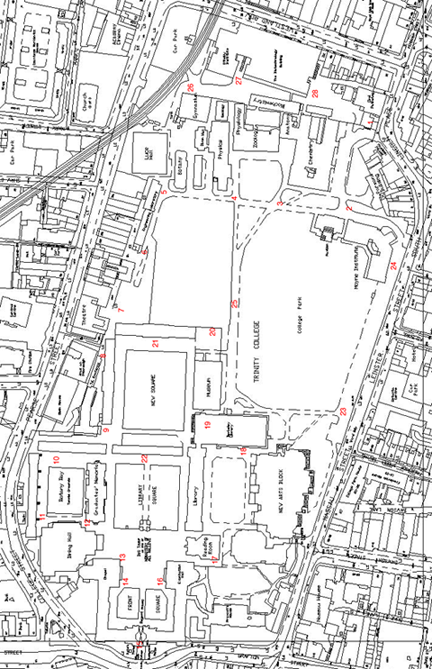
\includegraphics{tcd-survey.png}

\caption{All 28 survey points in TCD}

\end{figure}

\subsection{Survey Data}

\begin{tabular}{|c|c|c|c|c|c|c|}
\hline
Location	&	&	NetMonitor Menu	&	Cell ID	&	Signal Strength	& C2 Value	& Comments	\\
\hline
1	&		&	 3	&	732	&	33 - 66	&	45	&		\\
 	&		&	 4	&	103	&	27 - 78	&	27	&		\\
 	&		&	 5	&	746	&	15 - 83	&	26	&		\\
\hline	
2	&		&	 3	&	728	&	24 - 75	&	35	&	Signal Loss	\\
 	&		&	 4	&	117	&	31 - 73	&	37	&		\\
 	&		&	 5	&	100	&	27 - 78	&	27	&		\\
\hline	
3	&		&	 3	&	107	&	55 - 50	&	50	&		\\
 	&		&	 4	&	105	&	32 - 73	&	32	&		\\
 	&		&	 5	&	738	&	 9 - 90	&	23	&		\\
\hline	
4	&		&	 3	&	107	&	53 - 50	&	50	&	1 Mast Site \\
 	&		&	 4	&	728	&	32 - 73	&	32	&	Visible.		\\
 	&		&	 5	&	105	&	26 - 79	&	26	&	See Figure 2 \\
\hline	
5	&		&	 3	&	728	&	47 - 51	&	61	&	3 Mast Sites	\\
 	&		&	 4	&	110	&	51 - 54	&	48	&	Visible.	  		\\
 	&		&	 5	&	117	&	38 - 67	&	38	&	See Figures 3 - 5\\
\hline	
6	&		&	 3	&	732	&	33 - 66	&	45	&	2 Mast Site	\\
 	&		&	 4	&	103	&	27 - 78	&	27	&	Visible.	  	\\
 	&		&	 5	&	746	&	15 - 83	&	26	&	See Figures 3 - 4 \\
\hline	
7	&		&	 3	&	107	&	63 - 40	&	66	&	1 Mast Site	\\
 	&		&	 4	&	732	&	33 - 66	&	43	&	Visible.	  	\\
 	&		&	 5	&	100	&	26 - 79	&	31	&	See Figures 5	\\
\hline	
8	&		&	 3	&	719	&	33 - 76	&	40	&		\\
 	&		&	 4	&	728	&	18 - 80	&	27	&		\\
 	&		&	 5	&	716	&	13 - 86	&	24	&		\\
\hline	
9	&		&	 3	&	719	&	48 - 51	&	64	&	4 Mast Site	\\
 	&		&	 4	&	723	&	31 - 68	&	45	&	Visible.	  	\\
 	&		&	 5	&	716	&	27 - 72	&	33	&	See Figures 6 - 8	\\
\hline	
10	&		&	 3	&	719	&	55 - 44	&	70	&	1 Mast Site	\\
 	&		&	 4	&	110	&	38 - 68	&	36	&	Visible.	  	\\
 	&		&	 5	&	716	&	 7 - 90	&	19	&	See Figure 8	\\
\hline	
11	&		&	 3	&	723	&	27 - 74	&	43	& Signal Loss \\
 	&		&	 4	&	100	&	39 - 66	&	39	& 1 Mast Site Visible \\
 	&		&	 5	&	739	&	18 - 81	&	25	& See Figure 9	\\
\hline	
12	&		&	 3	&	728	&	43 - 56	&	60	&2 x Signal Loss \\
 	&		&	 4	&	100	&	39 - 66	&	39	&		\\
 	&		&	 5	&	739	&	18 - 81	&	25	&		\\
\hline	
13	&		&	 3	&	110	&	25 - 49	&	56	&	 	\\
 	&		&	 4	&	730	&	33 - 66	&	42	&		\\
 	&		&	 5	&	107	&	32 - 74	&	31	&		\\
\hline	
\end{tabular}

\begin{tabular}{|c|c|c|c|c|c|c|}
\hline
Location	&	&	NetMonitor Menu	&	Cell ID	&	Signal Strength	& C2 Value	& Comments	\\
\hline
14	&		&	 3	&	110	&	48 - 58	&	47	& 1 Mast Site \\
 	&		&	 4	&	117	&	34 - 71	&	34	& Visible	\\
 	&		&	 5	&	723	&	23 - 76	&	37	& See Figure 10	\\
\hline	
15	&		&	 3	&	739	&	48 - 51	&	58	& Signal Loss \\
 	&		&	 4	&	717	&	38 - 61	&	48	& 2 Mast Sites Visible \\
 	&		&	 5	&	113	&	38 - 65	&	40	& 	\\
\hline	
16	&		&	 3	&	110	&	42 - 66	&	38	&Signal Loss \\
 	&		&	 4	&	723	&	29 - 70	&	47	&		\\
 	&		&	 5	&	106	&	32 - 73	&	33	&		\\
\hline	
17	&		&	 3	&	728	&	51 - 48	&	60	&		\\
 	&		&	 4	&	738	&	38 - 61	&	48	&		\\
 	&		&	 5	&	100	&	31 - 74	&	31	&		\\
\hline	
18	&		&	 3	&	110	&	40 - 66	&	39	& 2 x Signal Loss \\
 	&		&	 4	&	738	&	30 - 76	&	33	&		\\
 	&		&	 5	&	732	&	17 - 81	&	28	&		\\
\hline	
19	&		&	 3	&	719	&	27 - 74	&	43	& Signal Loss \\
 	&		&	 4	&	110	&	39 - 66	&	39	&		\\
 	&		&	 5	&	107	&	33 - 75	&	30	&		\\
\hline	
20	&		&	 3	&	107	&	51 - 53	&	43	& 		\\
 	&		&	 4	&	100	&	20 - 79	&	34	&		\\
 	&		&	 5	&	739	&	17 - 82	&	23	&		\\
\hline	
21	&		&	 3	&	107	&	48 - 57	&	47	&		\\
 	&		&	 4	&	719	&	27 - 71	&	42	&		\\
 	&		&	 5	&	113	&	27 - 79	&	26	&		\\
\hline	
22	&		&	 3	&	719	&	41 - 58	&	73	&Signal Loss \\
 	&		&	 4	&	728	&	27 - 72	&	38	&		\\
 	&		&	 5	&	100	&	24 - 81	&	24	&		\\
\hline	
23	&		&	 3	&	107	&	55 - 48	&	57	&Signal Loss \\
 	&		&	 4	&	110	&	38 - 67	&	37	&		\\
 	&		&	 5	&	738	&	27 - 72	&	34	&		\\
\hline	
24	&		&	 3	&	107	&	60 - 43	&	63	&	 	\\
 	&		&	 4	&	110	&	28 - 82	&	23	&		\\
 	&		&	 5	&	719	&	15 - 84	&	29	&		\\
\hline	
25	&		&	 3	&	716	&	60 - 40	&	69	&Signal Loss \\
 	&		&	 4	&	100	&	36 - 69	&	35	&		\\
 	&		&	 5	&	110	&	34 - 21	&	38	&		\\
\hline	
26	&		&	 3	&	746	&	52 - 46	&	65	&		\\
 	&		&	 4	&	105	&	36 - 69	&	37	&		\\
 	&		&	 5	&	740	&	20 - 79	&	26	&		\\
\hline	
27	&		&	 3	&	101	&	37 - 68	&	40	&Signal Loss \\
 	&		&	 4	&	785	&	28 - 71	&	38	&		\\
 	&		&	 5	&	740	&	22 - 79	&	30	&		\\
\hline	
28	&		&	 3	&	105	&	30 - 69	&	38	&		\\
 	&		&	 4	&	746	&	20 - 75	&	34	&		\\
 	&		&	 5	&	110	&	-99 - 82	&	-99	&		\\
\hline
\end{tabular}

\subsection{Mobile Masts Noted}

Please see figures 2 - 10.

\begin{figure}[h]

\includegraphics{1.png}

\caption{Pearse St Fire Station Tower}

\end{figure}

\begin{figure}[h]

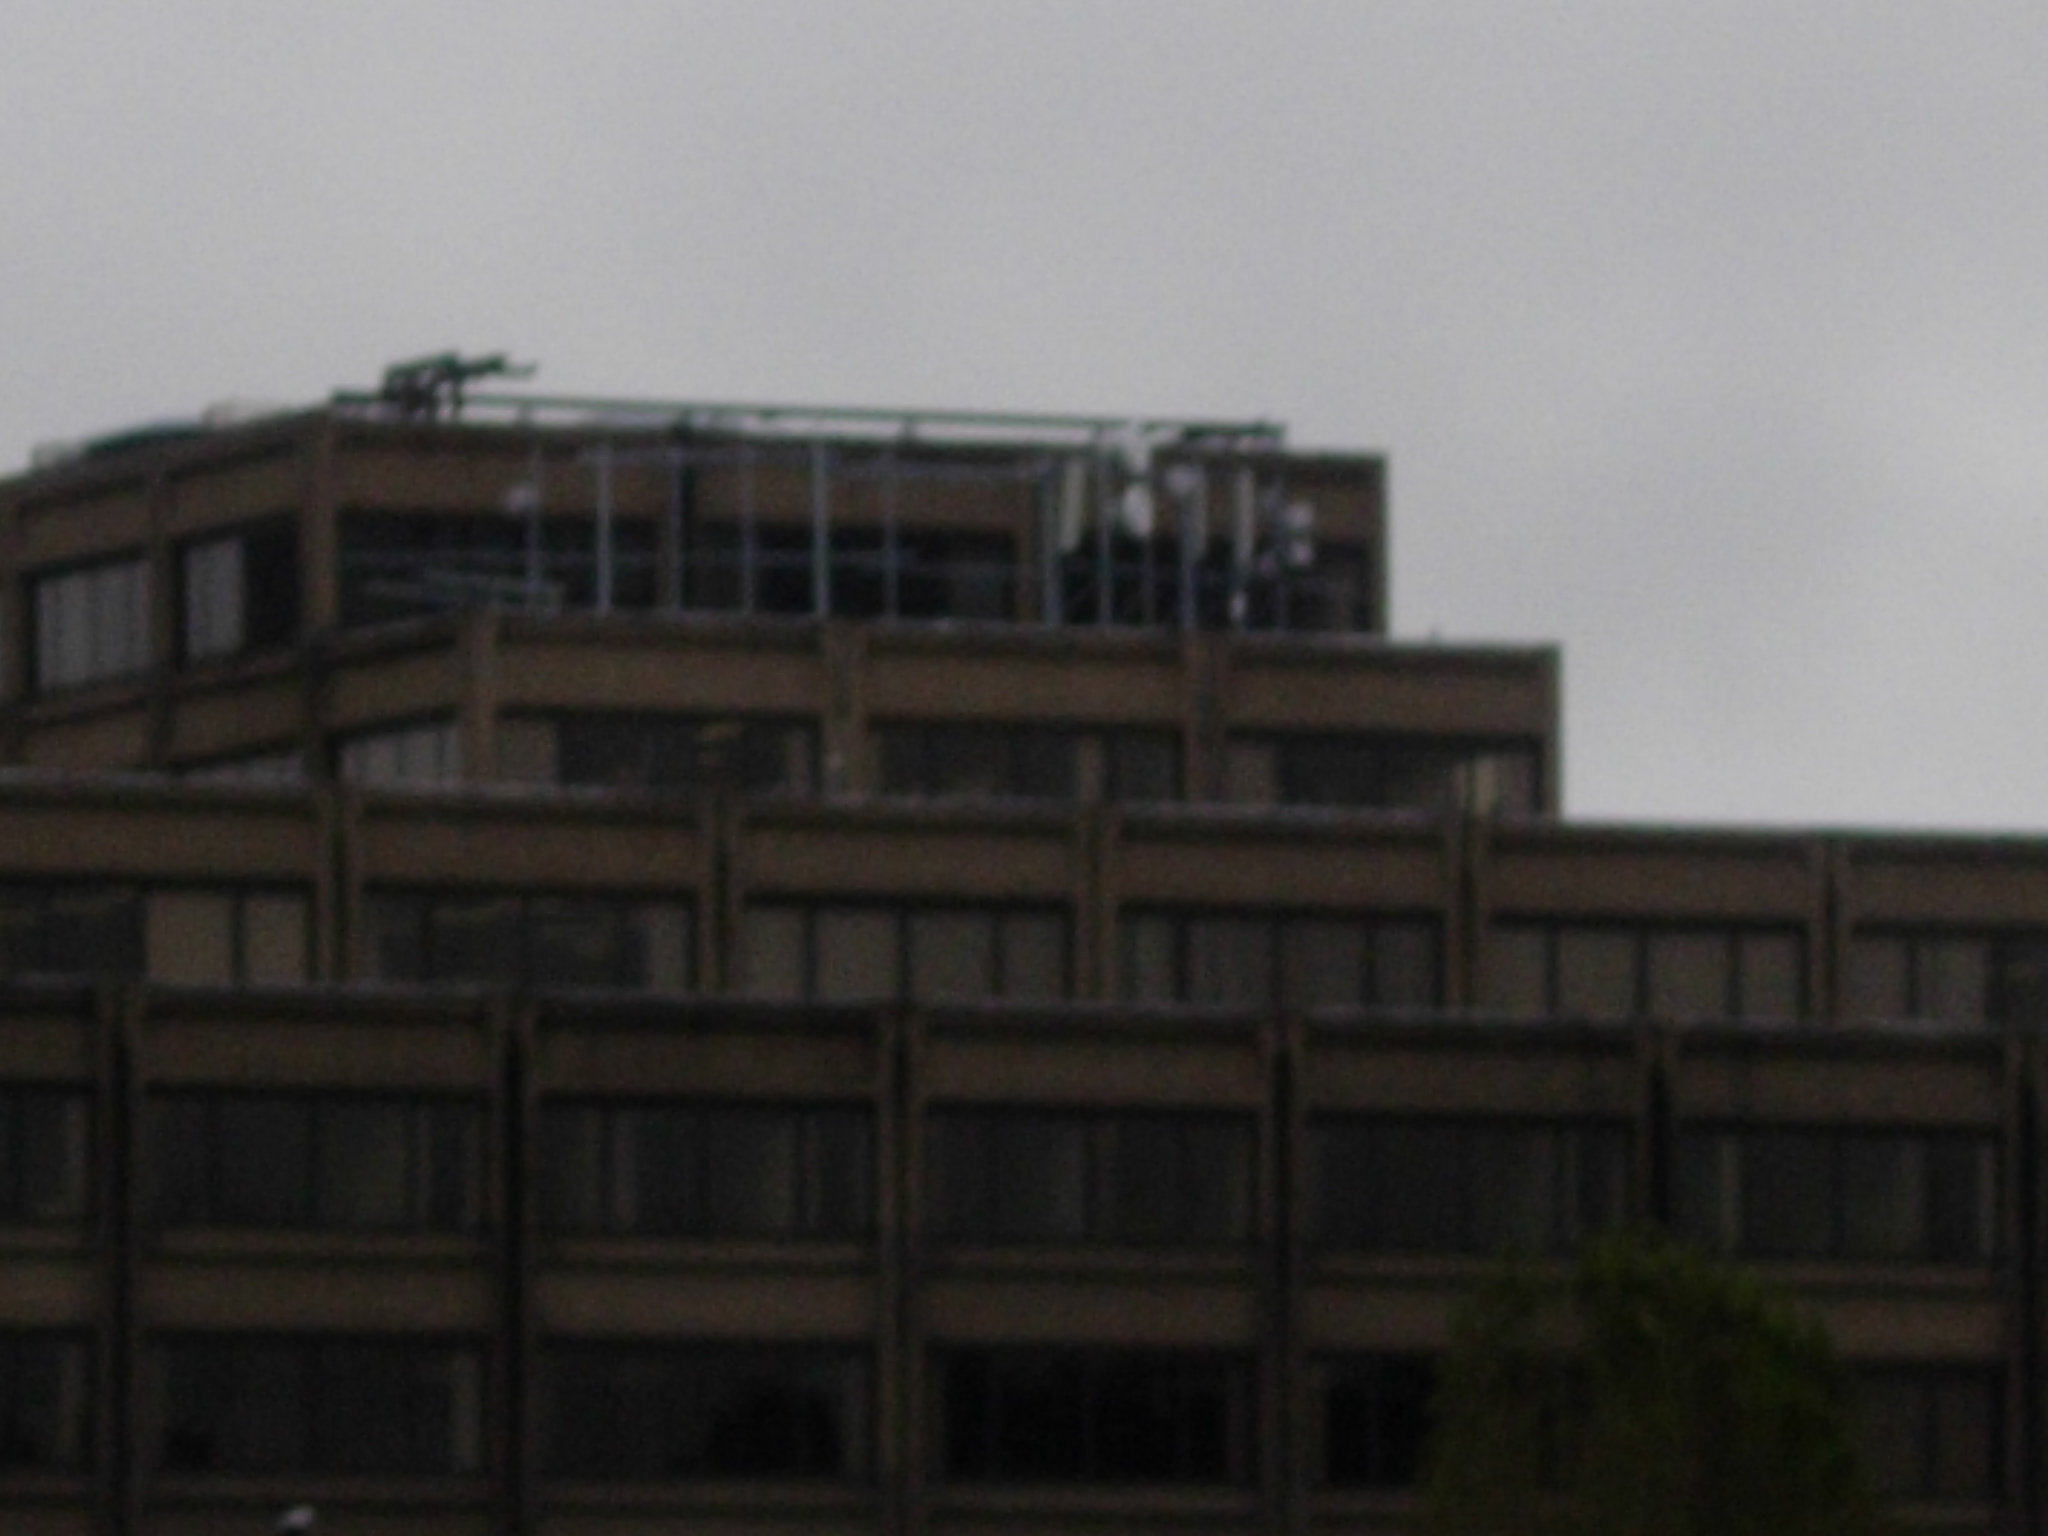
\includegraphics{2.png}

\caption{Roof along Nassau St}

\end{figure}

\begin{figure}[h]

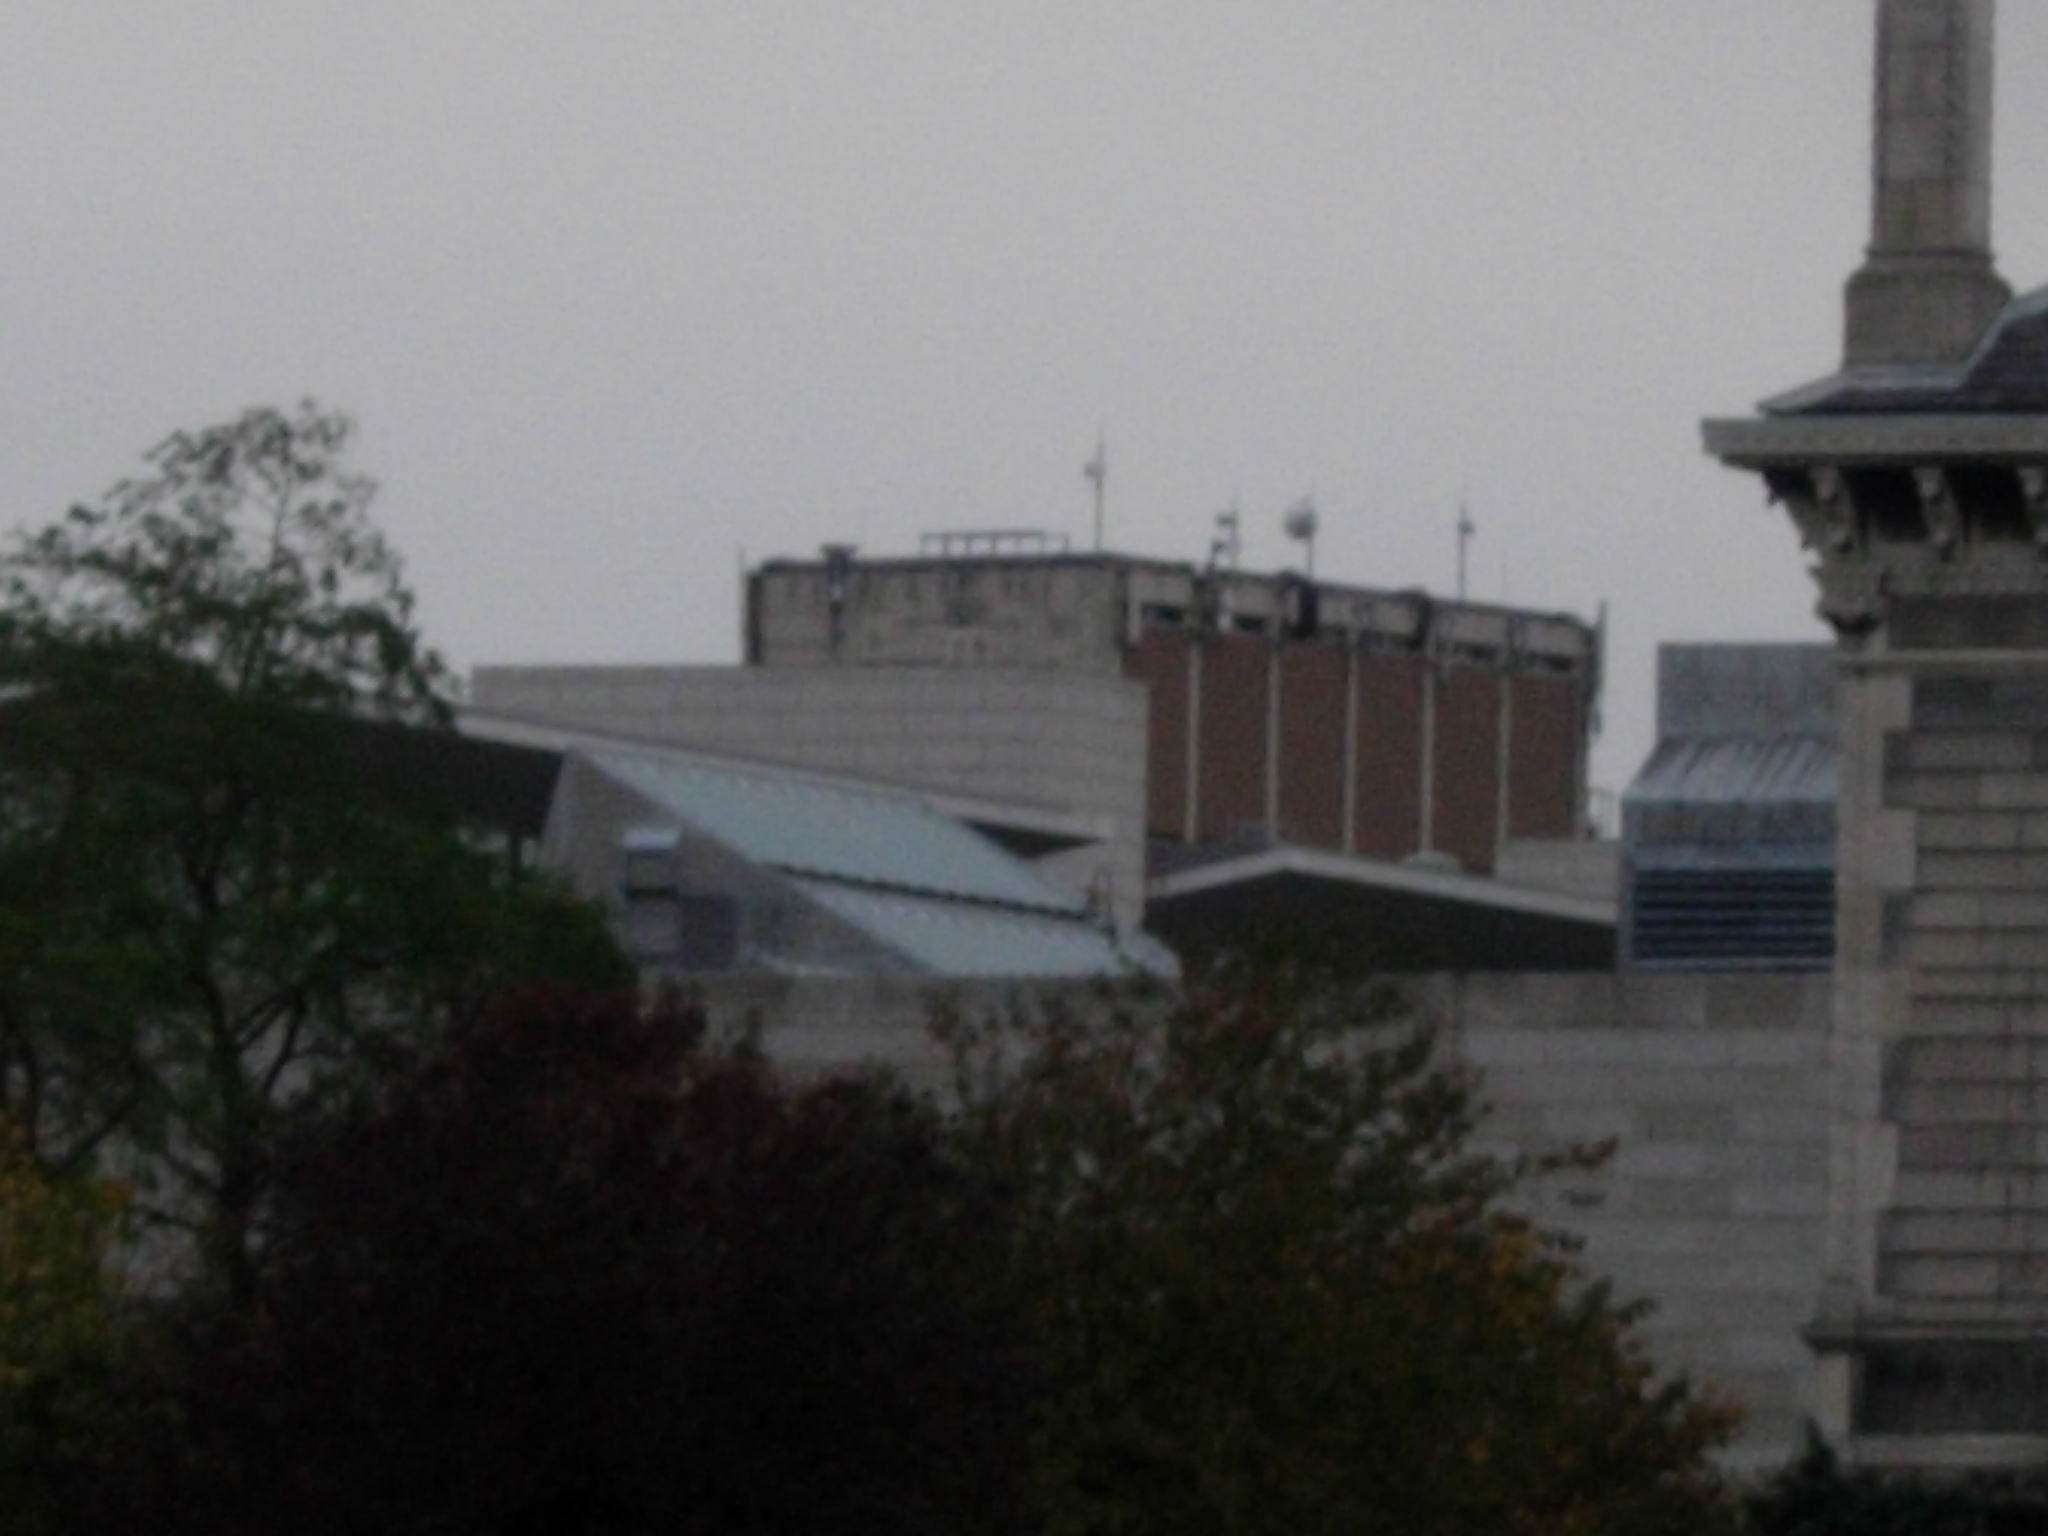
\includegraphics{5.png}

\caption{Nassau House}

\end{figure}

\begin{figure}[h]

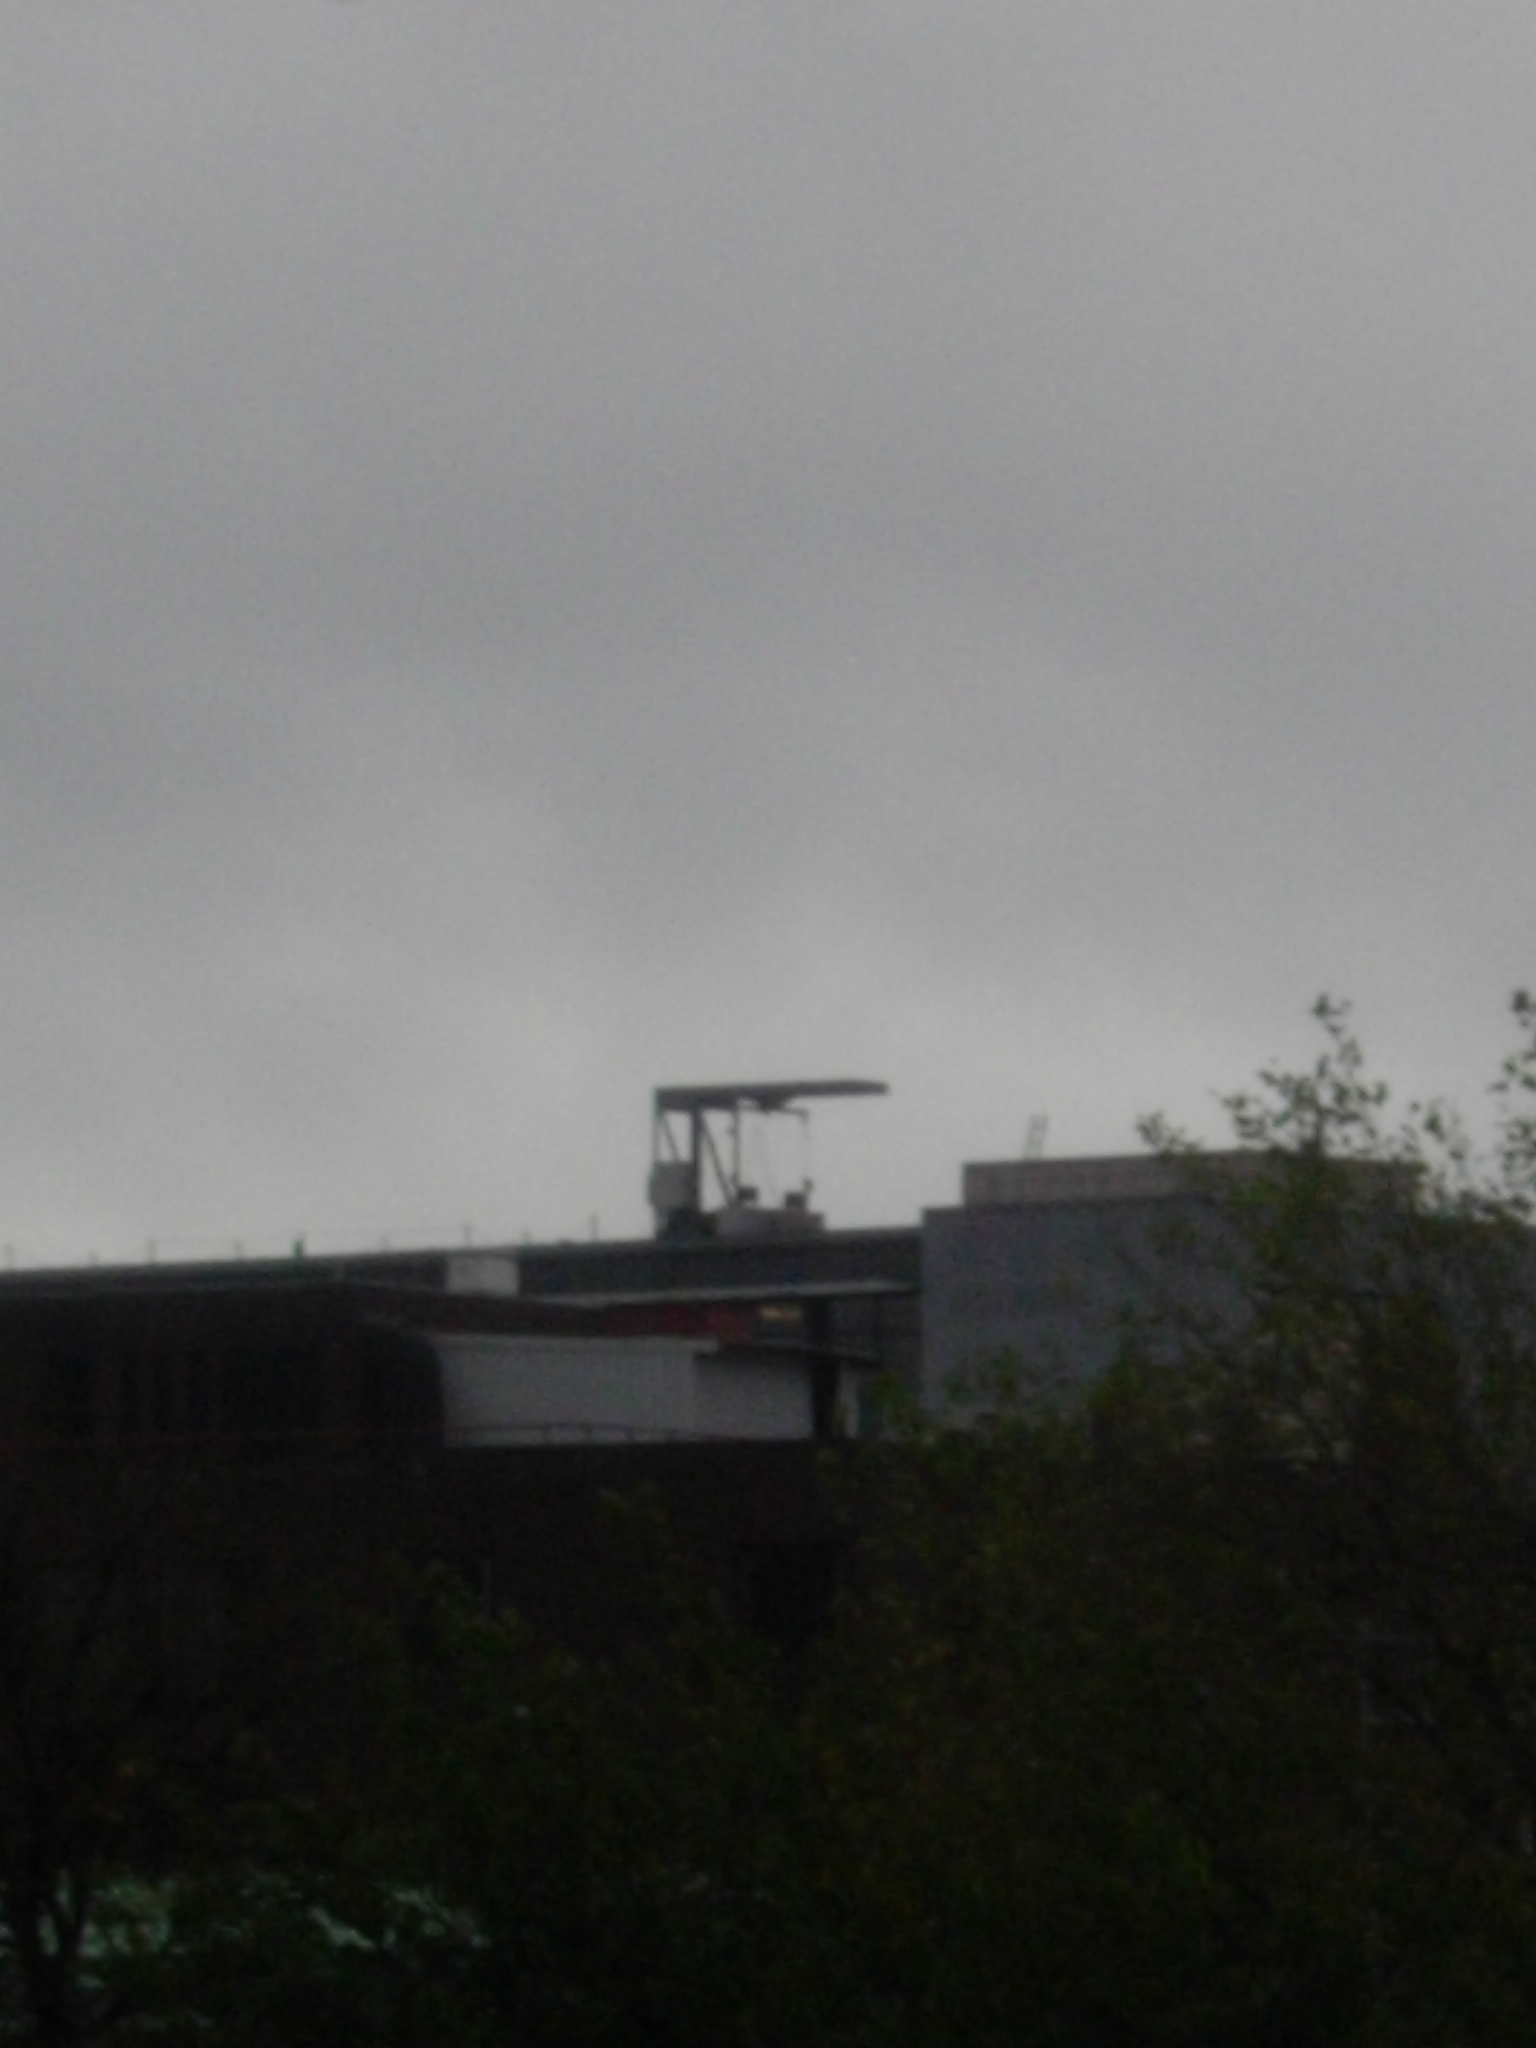
\includegraphics{6.png}

\caption{Buildings at corner of Nassau St and Kildare St}

\end{figure}

\begin{figure}[h]

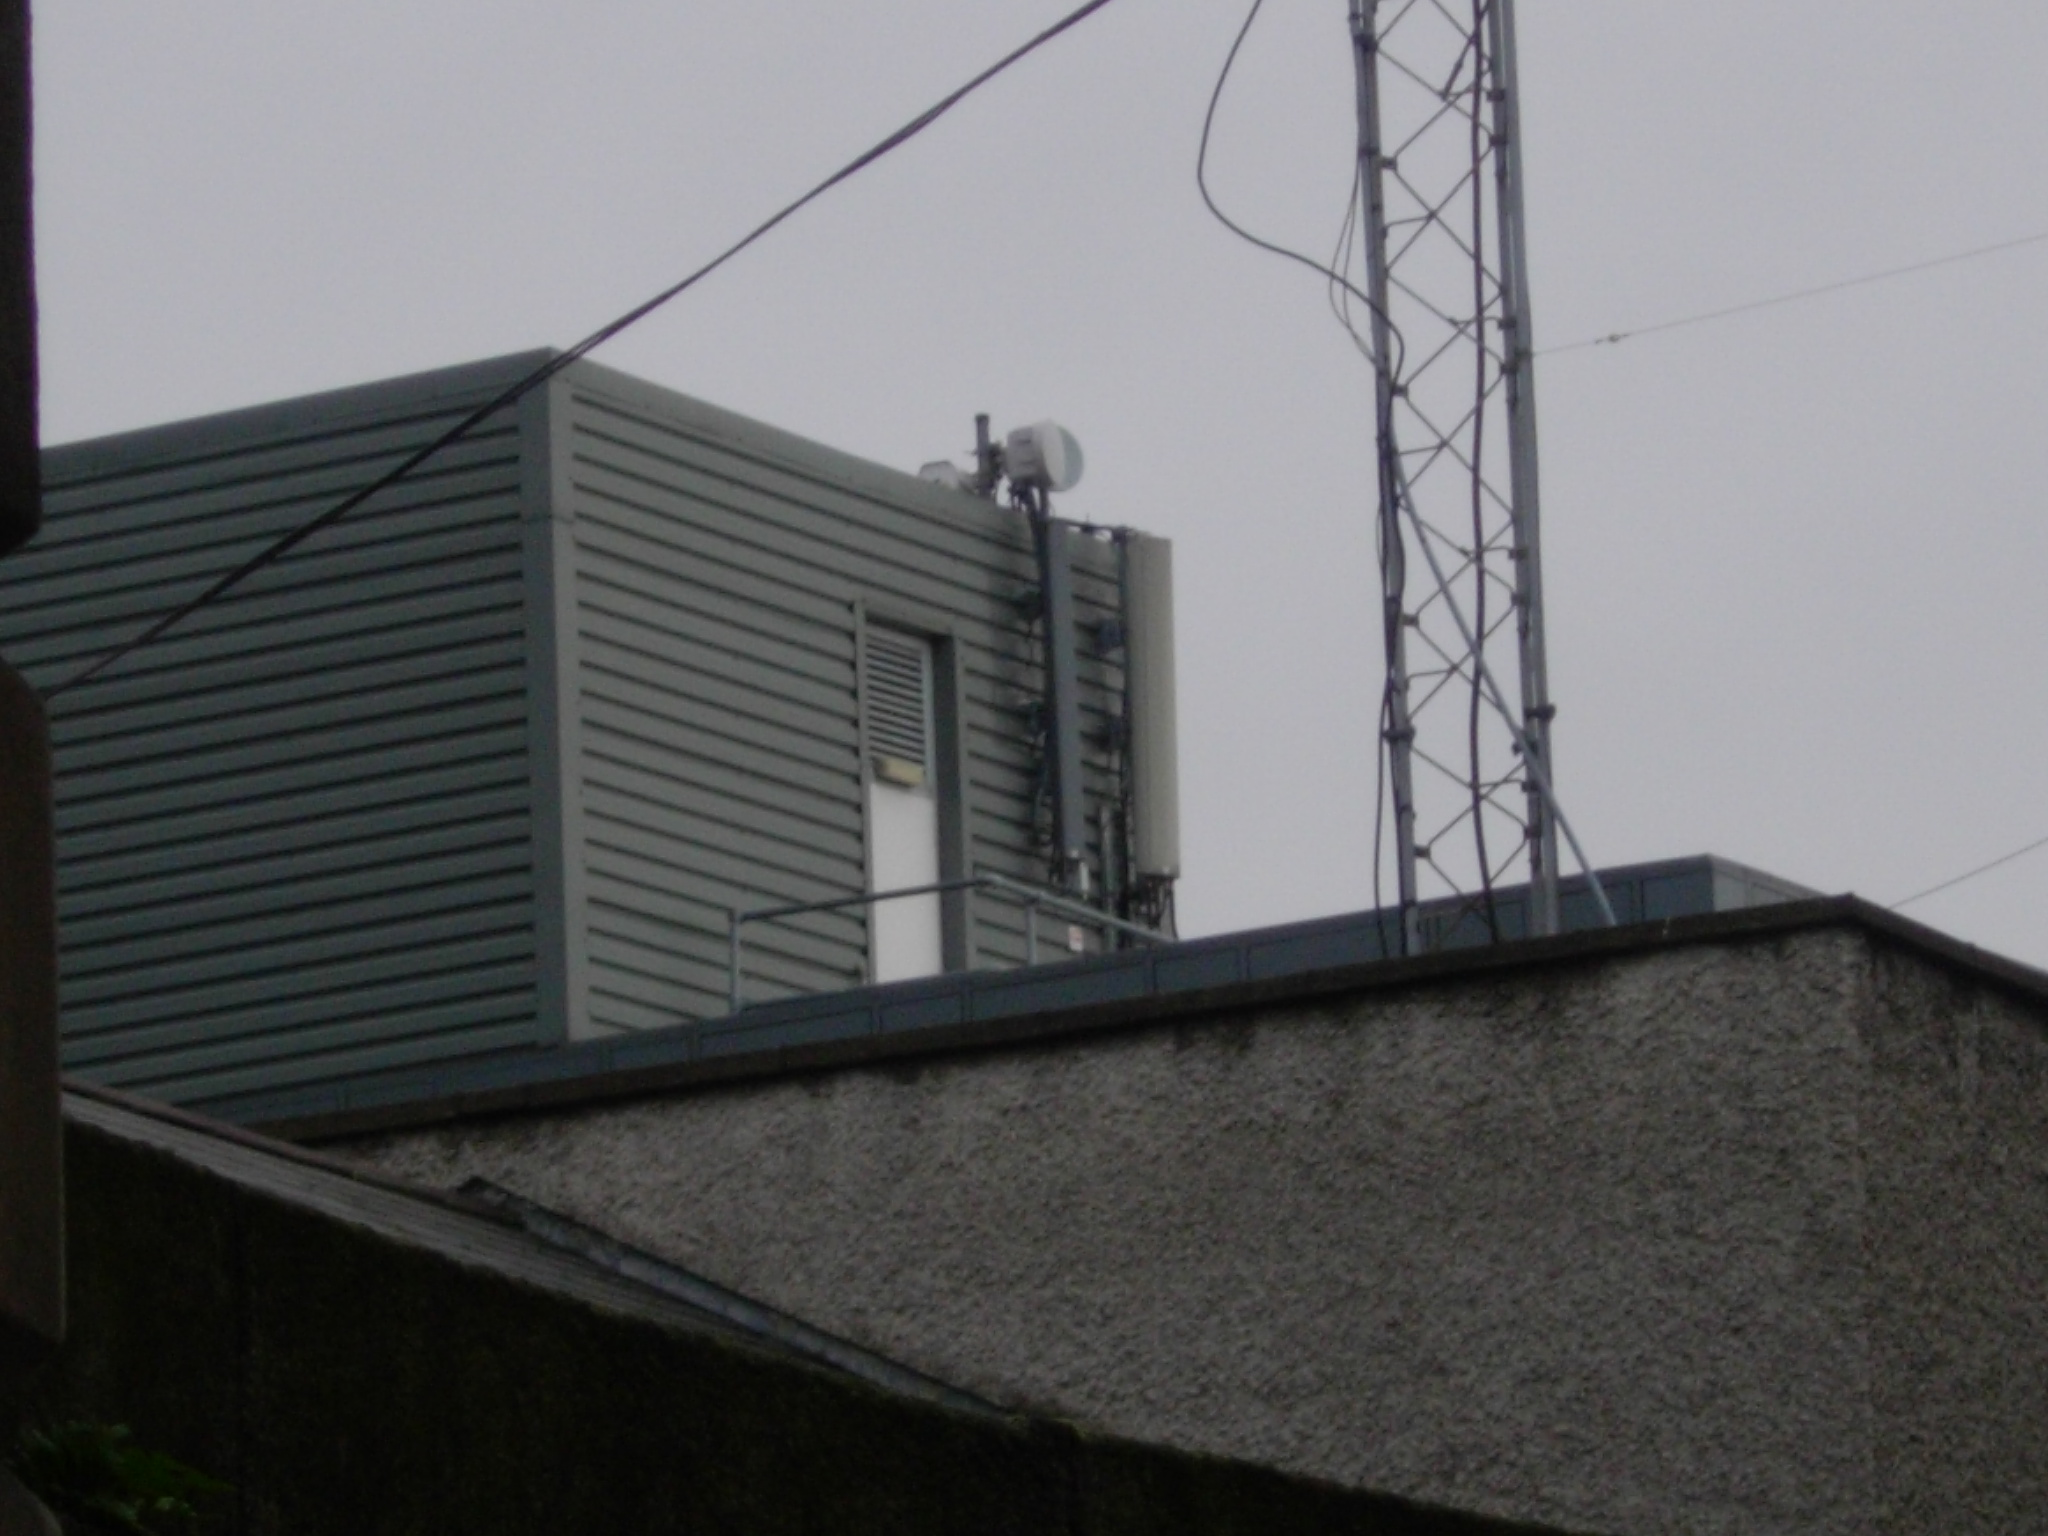
\includegraphics{7.png}

\caption{Roof of \'{A}ras an Phairsaigh}

\end{figure}

\begin{figure}[h]

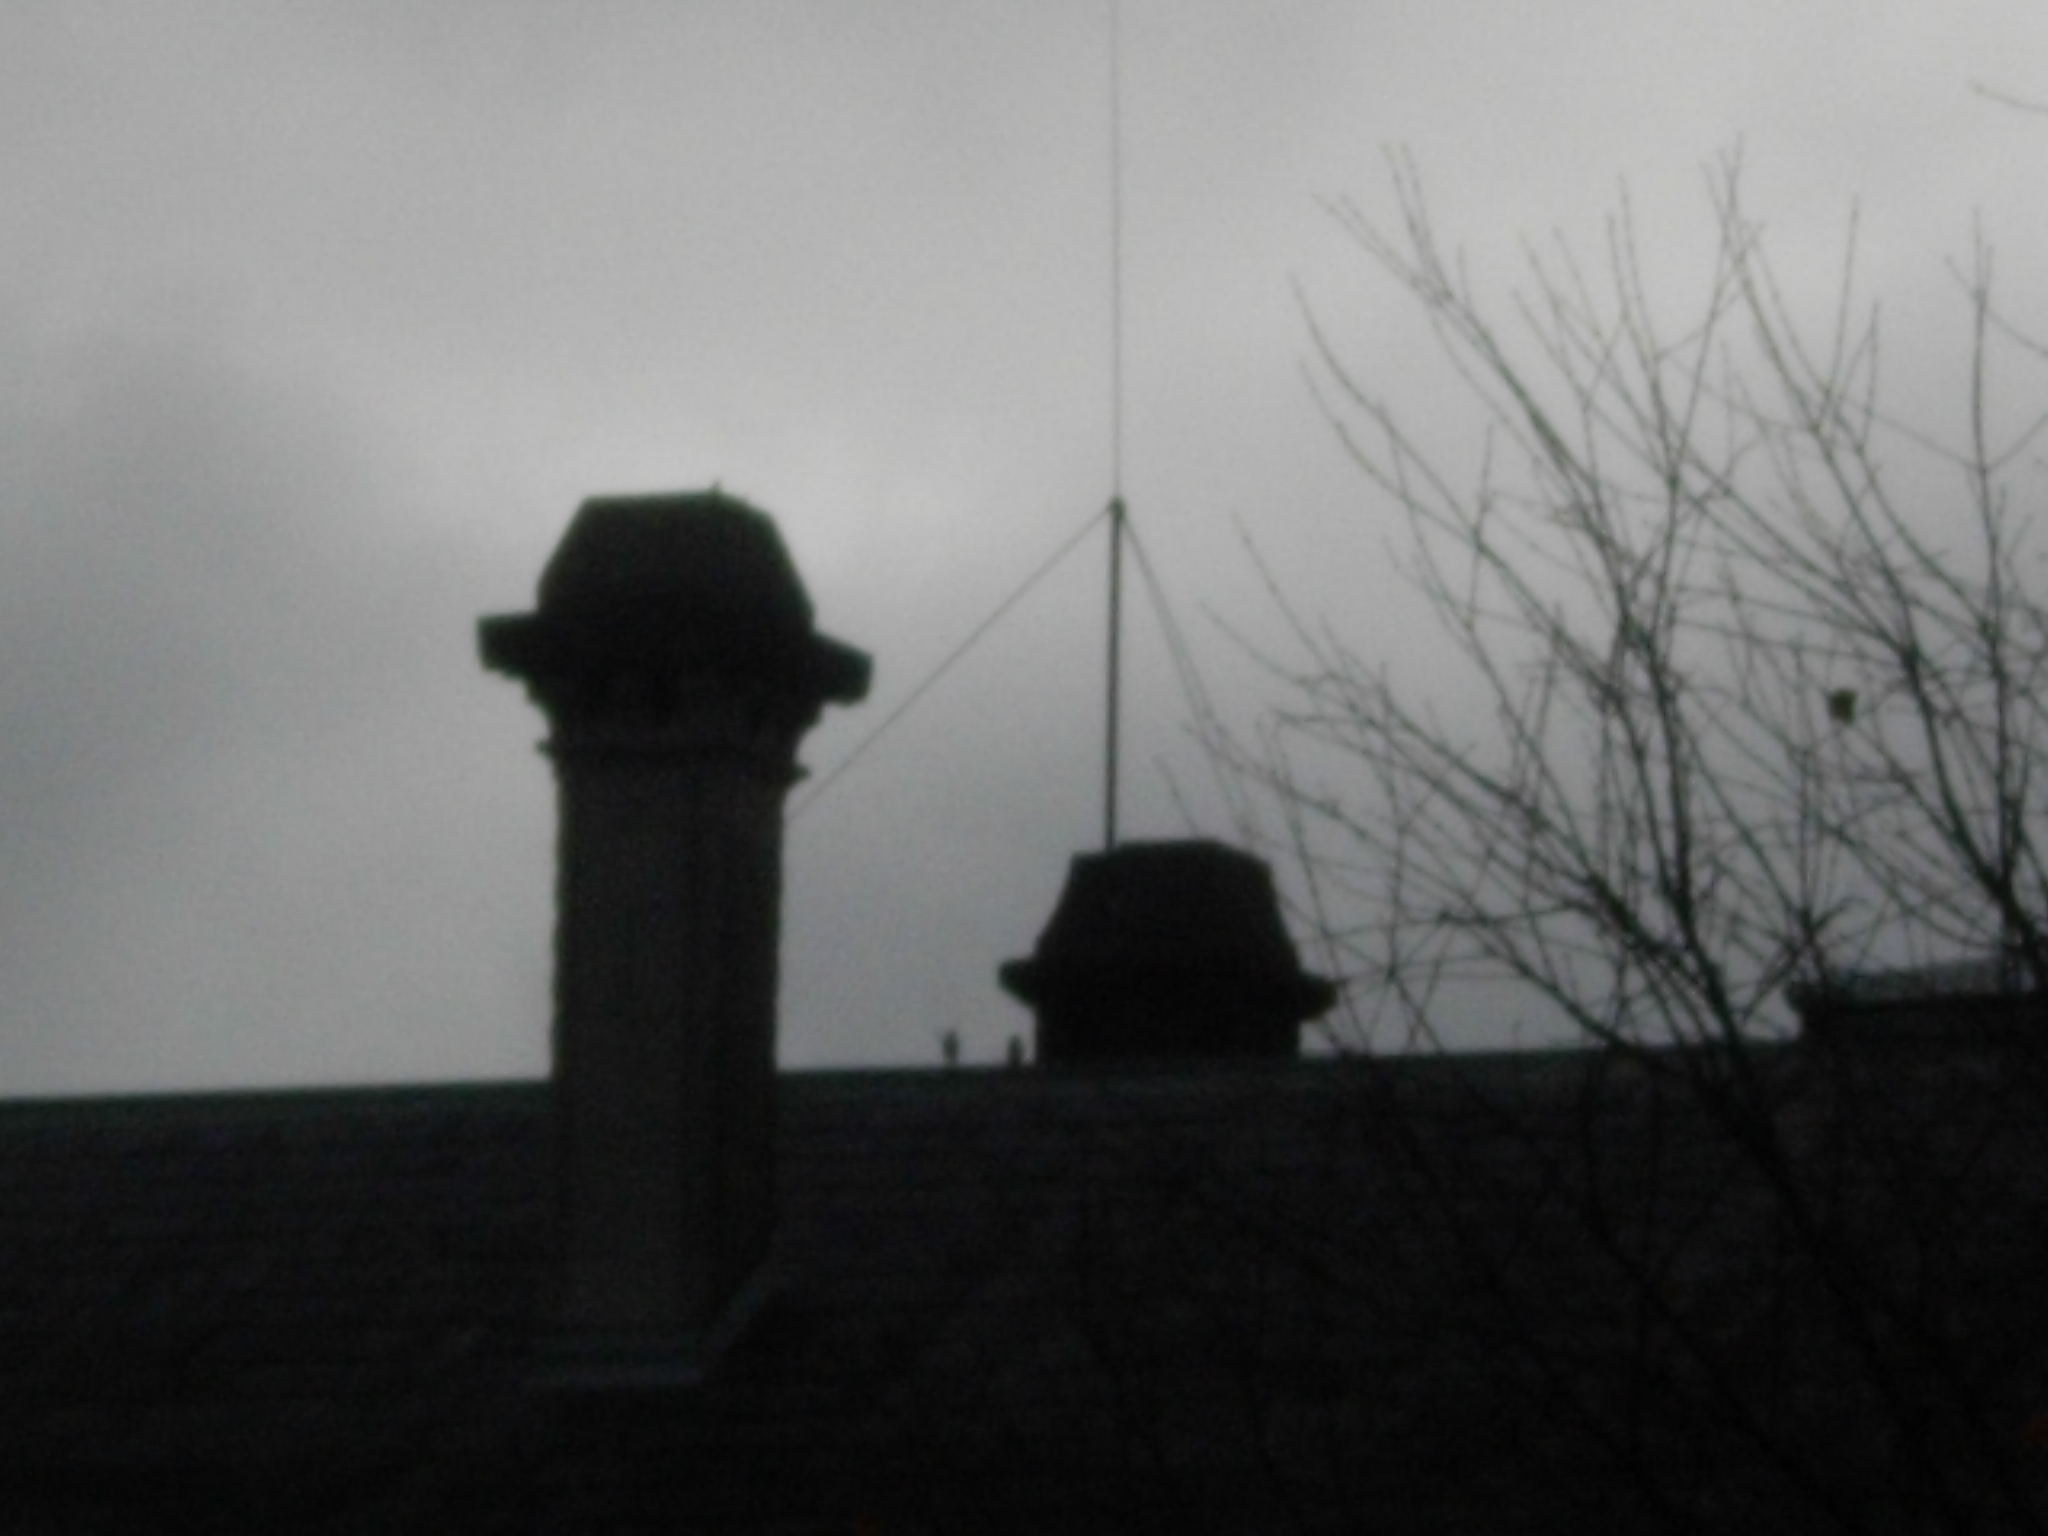
\includegraphics{8.png}

\caption{Roof of Museum Building}

\end{figure}

\begin{figure}[h]

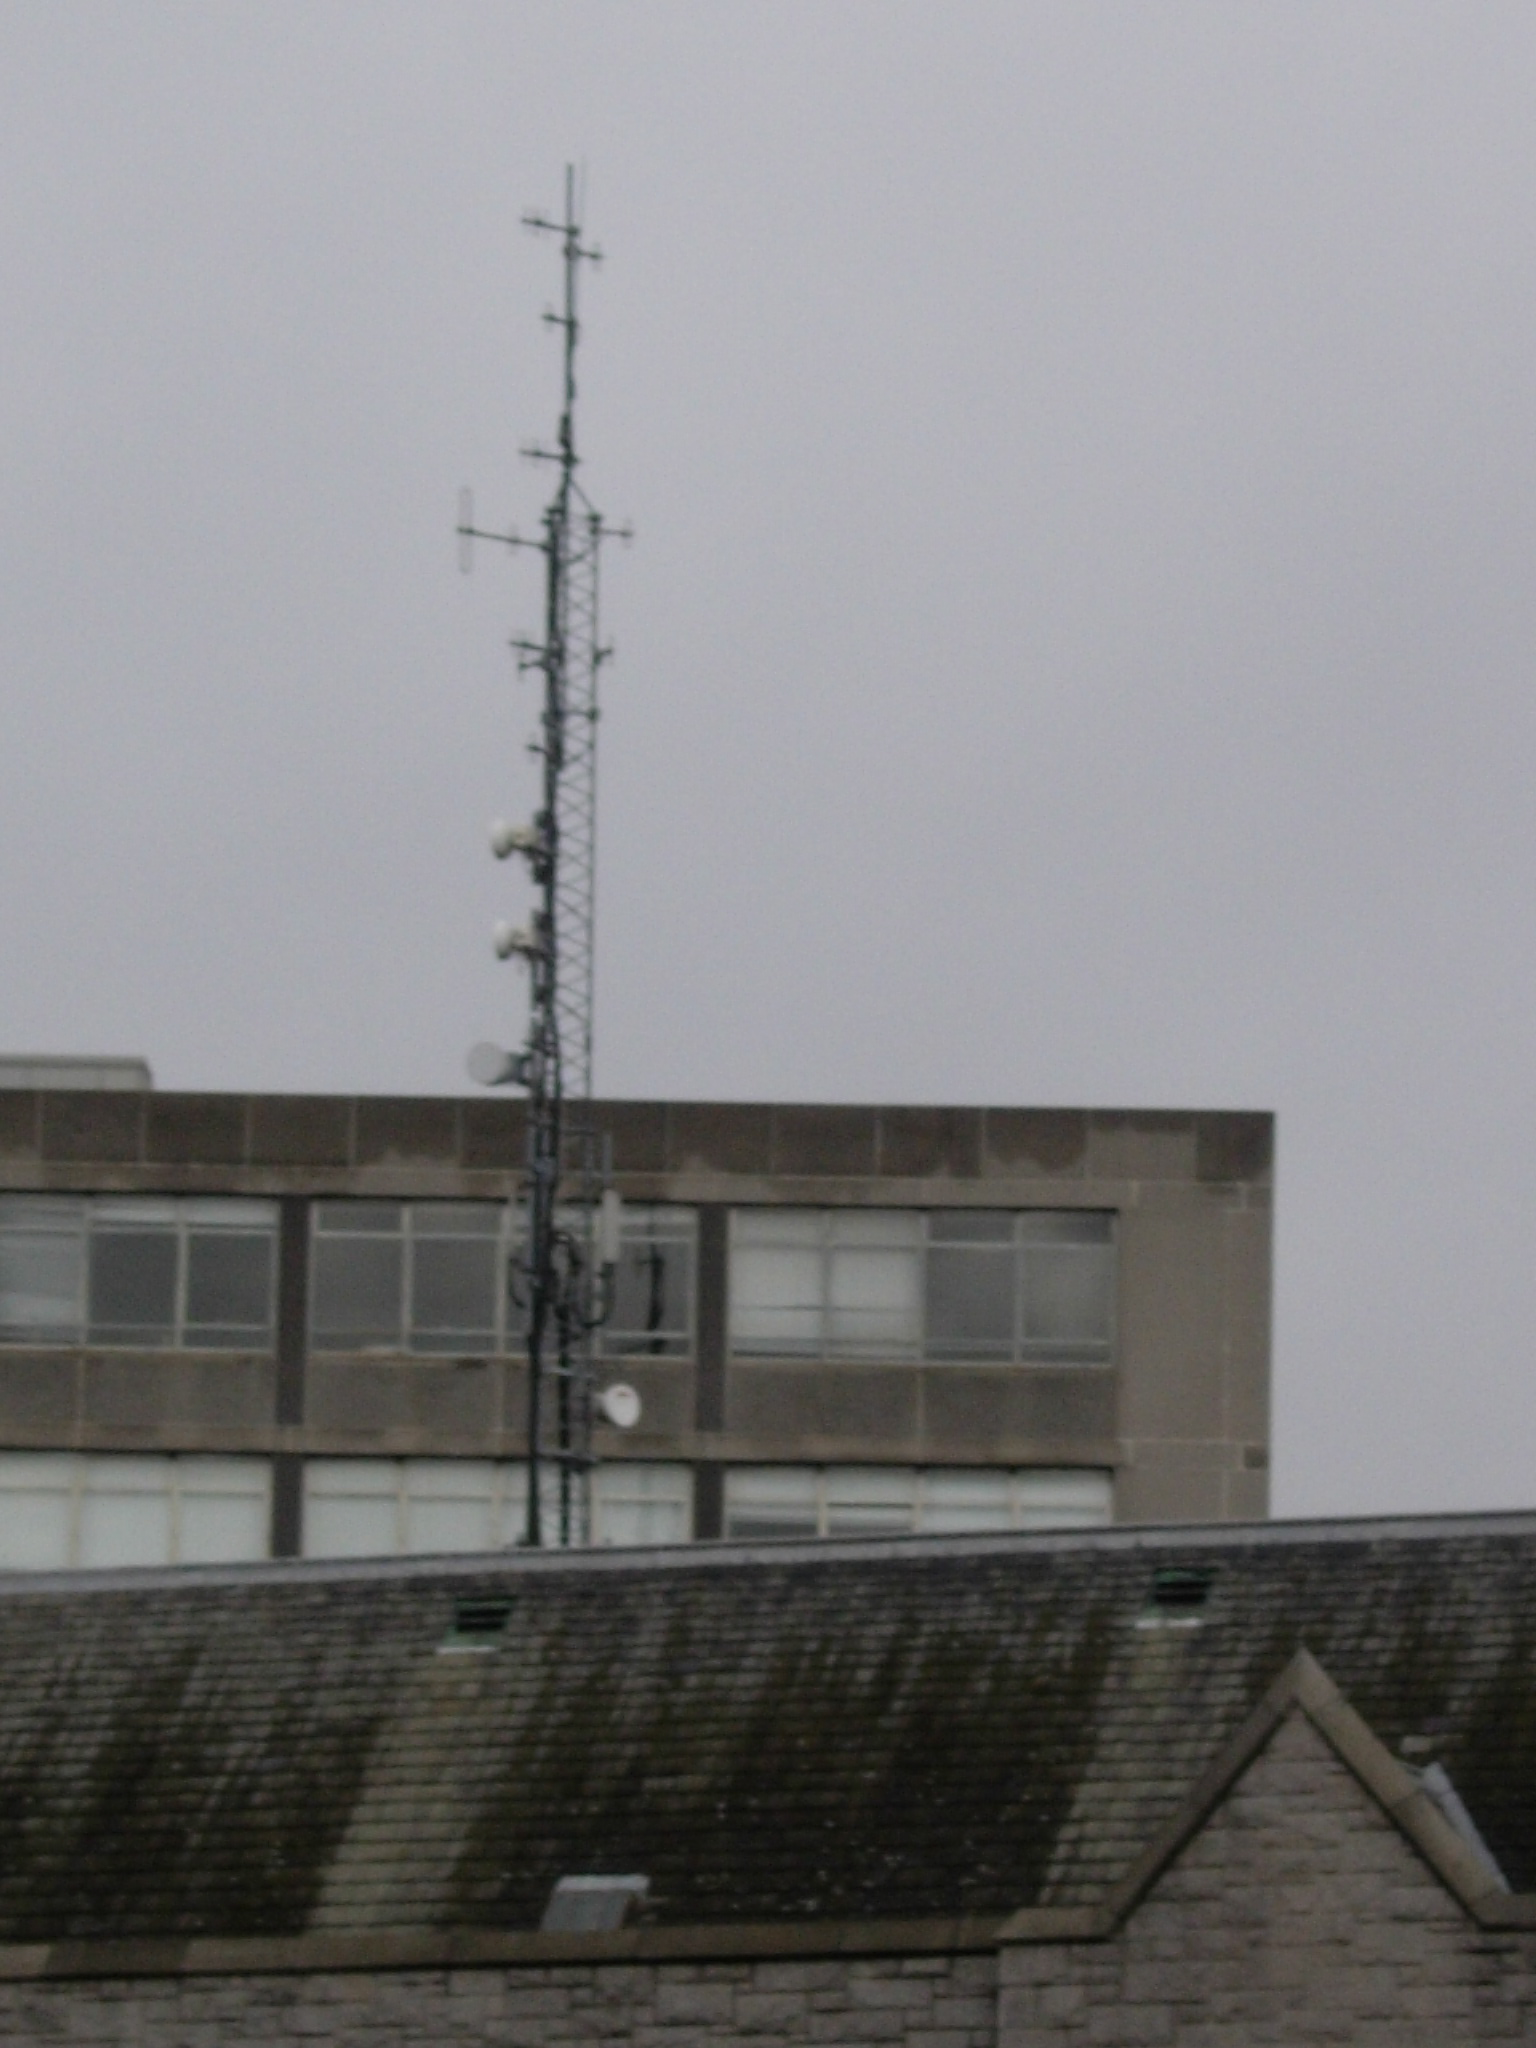
\includegraphics{9.png}

\caption{Roof of Pearse St Garda Station}

\end{figure}

\begin{figure}[h]

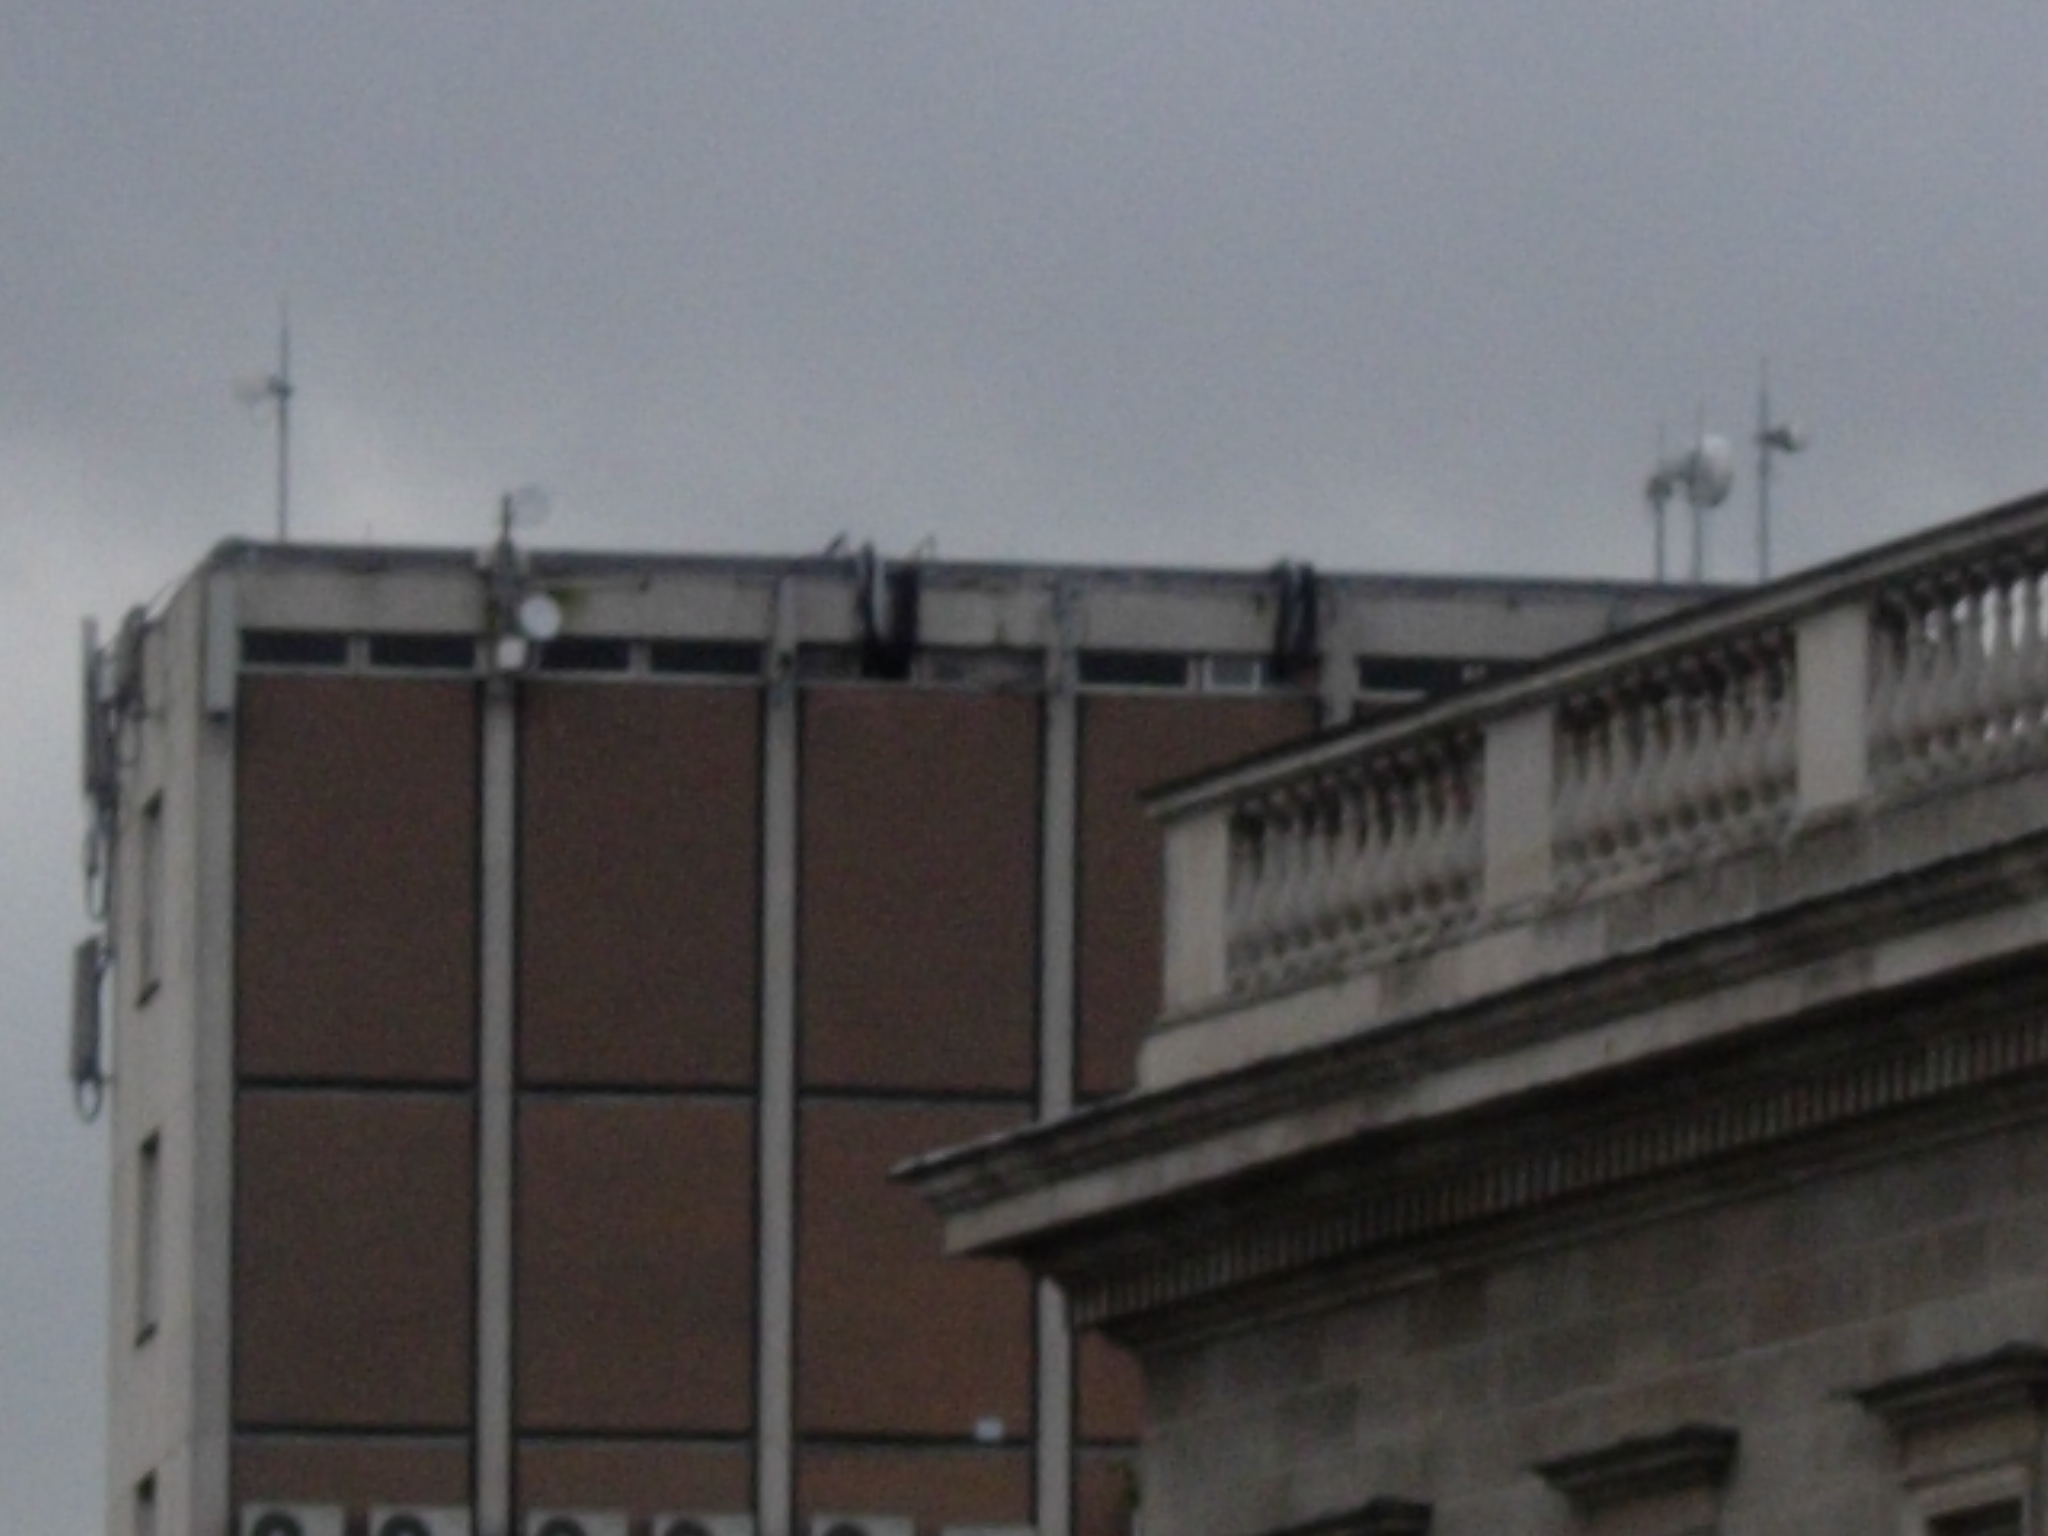
\includegraphics{11.png}

\caption{Roof of Nassau House}

\end{figure}

\begin{figure}[h]

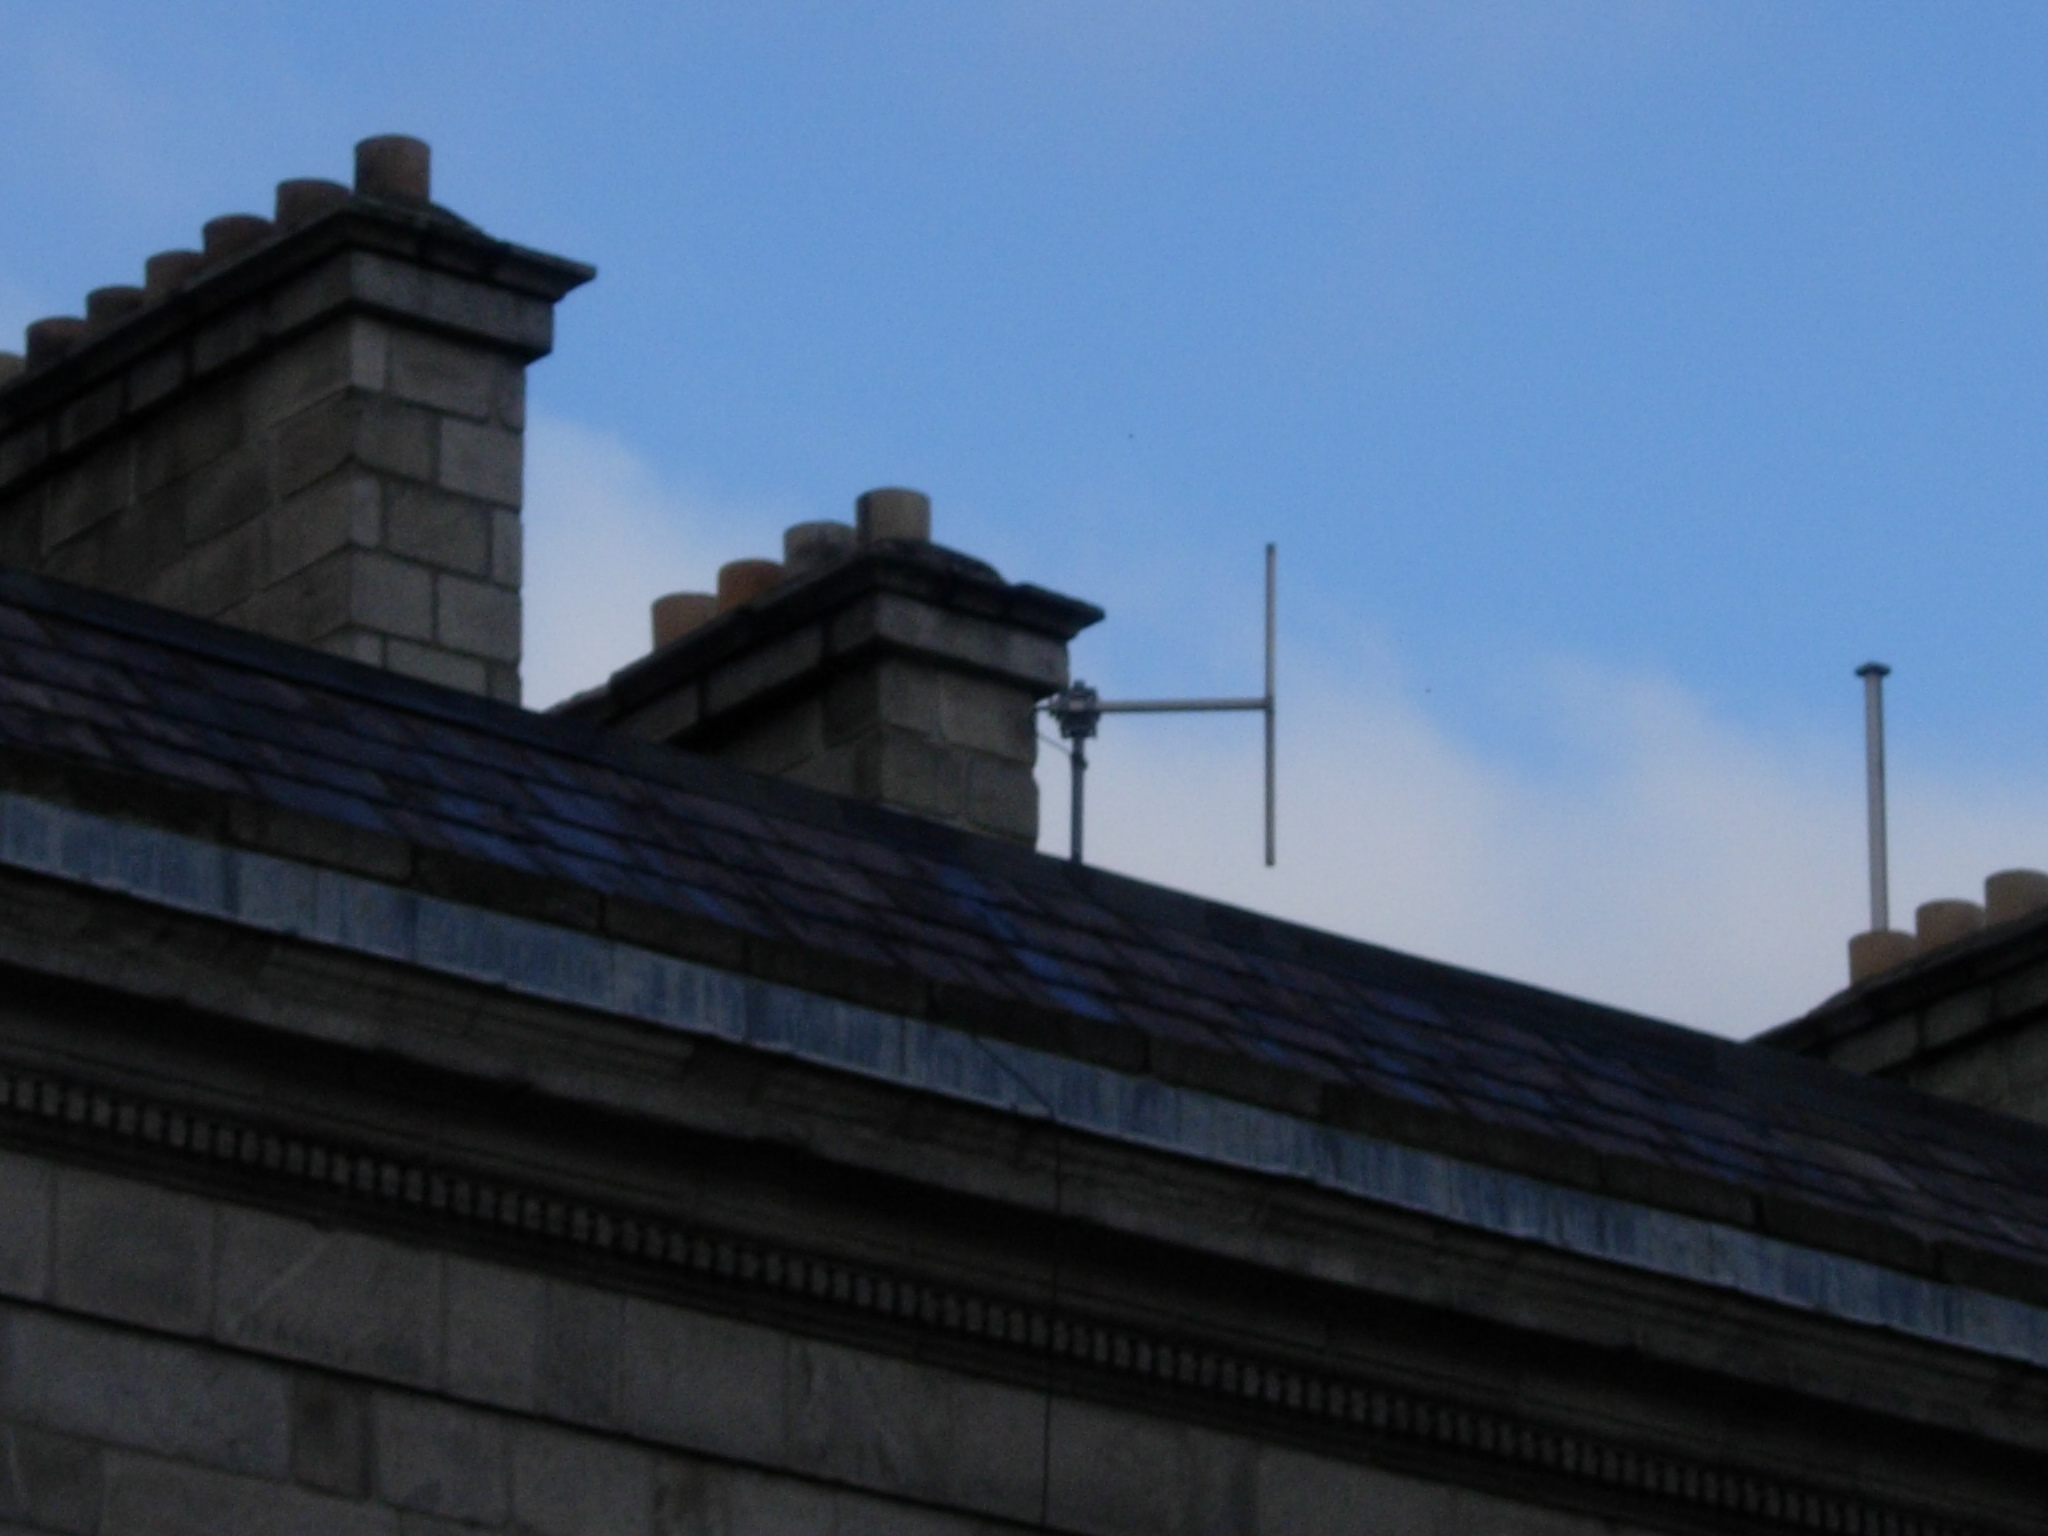
\includegraphics{12.png}

\caption{Roof of House 6}

\end{figure}

\subsection{Survey Comments}

While generating this report, I realised that I had made a fundamental
misunderstanding in interpreting the output of NetMonitor on the Nokia
3210. I failed to note down any cell details except for the serving
cell, the 3rd neighbour cell and the 6th neighbour cell. 


Had I realised this mistake prior to returning the Nokia 3210, I would
have attempted to conduct the surveying again to note down complete and
accurate readings. Hopefully, the large no of surveys I conducted in 
roughly even distances from each other will minimise the impact of this 
fatal mistake.

\section{Estimated Mobile Network}

\subsection{Map}

Please see figure 11.

\begin{figure}[h]

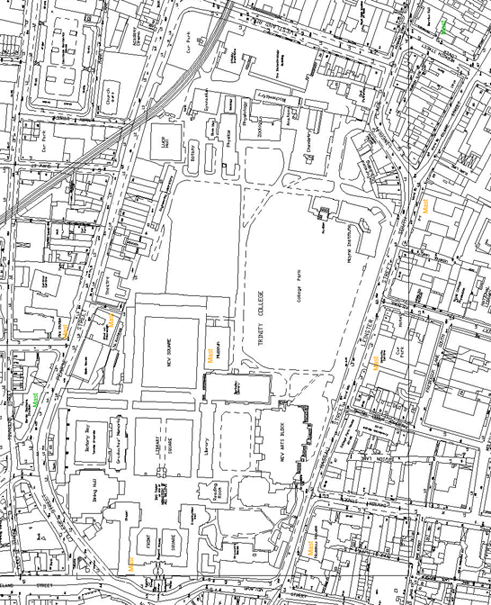
\includegraphics{tcd-masts.png}

\caption{Recorded Masts in Orange. Suspected O2 Masts in Green}

\end{figure}

\subsection{Justifying the Estimate}

There are 2 reasons why I believe despite the 9 mobile cell masks easily
identified on or adjacent to the TCD campus, only two of them are
connected to the O2 network.


The first mask location is based on previous knowledge. In the late 1990's,
Esat, now known as O2, made an agreement with An Gharda Siochana which
allowed for Esat/O2 to place mobile cell masks on numerous Gardai
stations around the country, in exchange for discounted mobile calls for
Gardai. Using this knowledge, I can deduce that the mobile mast visible
from the Pease St Gardai Station must be an O2 mast.


The second mask location is based upon empirical data during the survey.
The strongest signals being recorded once the Pearse St Garda Station
mast had been identified, were locations surveyed in proximity to
Westland Row and Lincoln Place were stronger. As a result, I believe the
masts identifiable on the roof of the Davenport Hotel are powering
additional cells on the O2 network.

\section{Conclusion}

Throughout my surveying, I only ever noticed cell ids between 100 - 117
and 716 - 785. Although I cannot prove it, I would assume these cell id
ranges indicate only 2 main concentrations of masts. Given that the
typical minimum radius of a cell is roughly 100m, the relatively small
area the TCD campus covers and the vast number of unique cell ids, I 
would conclude that O2 possess a large number of cells in the TCD 
area, providing multiple short distance cell coverage,
to ensure ample bandwidth for peak times.

\end{document}
